\chapter{احتمال}

\index{احتمال}

یک \key{احتمال} عددی حقیقی بین $0$ و $1$ است
که میزان محتمل بودن یک پیشامد را نشان می‌دهد.
اگر رخ دادن پیشامدی قطعی باشد،
احتمال آن 1 است،
و اگر پیشامدی غیرممکن باشد،
احتمال آن 0 است.
احتمال یک پیشامد با $P(\cdots)$ نشان داده می‌شود
که در آن سه نقطه پیشامد را توصیف می‌کند.

برای مثال، هنگام پرتاب یک تاس،
نتیجه یک عدد صحیح بین $1$ و $6$ است،
و احتمال هر نتیجه $1/6$ است.
برای مثال، می‌توانیم احتمال‌های زیر را محاسبه کنیم:

\begin{itemize}[noitemsep]
\item $P(\textrm{''نتیجه 4 باشد''})=1/6$
\item $P(\textrm{''نتیجه 6 نباشد''})=5/6$
\item $P(\textrm{''نتیجه زوج باشد''})=1/2$
\end{itemize}

\section{محاسبه}

برای محاسبه احتمال یک پیشامد،
می‌توانیم از ترکیبیات استفاده کنیم
یا فرآیندی را که پیشامد را تولید می‌کند شبیه‌سازی نماییم.
به عنوان مثال، بیایید احتمال کشیدن سه کارت با ارزش یکسان
از یک دسته کارت بر خورده را محاسبه کنیم
(برای مثال، $\spadesuit 8$، $\clubsuit 8$ و $\diamondsuit 8$).

\subsubsection*{روش ۱}

می‌توانیم احتمال را با استفاده از فرمول زیر محاسبه کنیم:

\[\frac{\textrm{تعداد پیشامدهای مطلوب}}{\textrm{تعداد کل پیشامدها}}.\]

در این مسئله، پیشامدهای مطلوب مواردی هستند
که در آن‌ها ارزش هر کارت یکسان است.
تعداد $13 {4 \choose 3}$ از این پیشامدها وجود دارد،
زیرا $13$ حالت ممکن برای ارزش کارت‌ها
و ${4 \choose 3}$ روش برای انتخاب $3$ خال از $4$ خال ممکن وجود دارد.

در مجموع ${52 \choose 3}$ برآمد وجود دارد،
زیرا ما 3 کارت از 52 کارت را انتخاب می‌کنیم.
بنابراین، احتمال پیشامد برابر است با:

\[\frac{13 {4 \choose 3}}{{52 \choose 3}} = \frac{1}{425}.\]

\subsubsection*{روش ۲}

روش دیگر برای محاسبه احتمال،
شبیه‌سازی فرآیندی است که پیشامد را تولید می‌کند.
در این مثال، سه کارت می‌کشیم، بنابراین فرآیند
شامل سه مرحله است.
لازم است که هر مرحله از فرآیند موفقیت‌آمیز باشد.

کشیدن اولین کارت قطعا موفقیت‌آمیز است،
زیرا هیچ محدودیتی وجود ندارد.
مرحله دوم با احتمال $3/51$ موفق می‌شود،
زیرا 51 کارت باقی مانده و 3 تا از آن‌ها
ارزشی یکسان با کارت اول دارند.
به طور مشابه، مرحله سوم با احتمال $2/50$ موفق می‌شود.

احتمال اینکه کل فرآیند موفقیت‌آمیز باشد برابر است با:

\[1 \cdot \frac{3}{51} \cdot \frac{2}{50} = \frac{1}{425}.\]

\section{پیشامدها}

یک پیشامد در نظریه احتمال می‌تواند به عنوان یک مجموعه نمایش داده شود:
\[A \subset X,\]
که در آن $X$ شامل همه برآمدهای ممکن است
و $A$ زیرمجموعه‌ای از برآمدهاست.
برای مثال، هنگام پرتاب یک تاس، برآمدها عبارتند از:
\[X = \{1,2,3,4,5,6\}.\]
حال، به عنوان مثال، پیشامد ''نتیجه زوج باشد''
متناظر با مجموعه زیر است:
\[A = \{2,4,6\}.\]

به هر برآمد $x$ یک احتمال $p(x)$ نسبت داده می‌شود.
سپس، احتمال $P(A)$ برای یک پیشامد
$A$ را می‌توان به صورت مجموع
احتمال‌های برآمدها با استفاده از فرمول زیر محاسبه کرد:
\[P(A) = \sum_{x \in A} p(x).\]
به عنوان مثال، هنگام پرتاب یک تاس،
برای هر برآمد $x$ داریم $p(x)=1/6$،
بنابراین احتمال پیشامد
«برآمد زوج است» برابر است با:
\[p(2)+p(4)+p(6)=1/2.\]

مجموع احتمال برآمدهای موجود در $X$ باید
برابر با ۱ باشد، یعنی $P(X)=1$.

از آنجا که پیشامدها در نظریه احتمالات مجموعه‌ هستند،
می‌توانیم با استفاده از عملگرهای استاندارد مجموعه‌ها روی آن‌ها عملیات انجام دهیم:

\begin{itemize}
\item \key{متمم} $\bar A$ یعنی
«$A$ رخ ندهد».
به عنوان مثال، هنگام پرتاب تاس،
متمم $A=\{2,4,6\}$ برابر است با
$\bar A = \{1,3,5\}$.
\item \key{اجتماع} $A \cup B$ یعنی
«$A$ یا $B$ رخ دهد».
به عنوان مثال، اجتماع
$A=\{2,5\}$
و $B=\{4,5,6\}$ برابر است با
$A \cup B = \{2,4,5,6\}$.
\item \key{اشتراک} $A \cap B$ یعنی
«$A$ و $B$ رخ دهند».
به عنوان مثال، اشتراک
$A=\{2,5\}$ و $B=\{4,5,6\}$ برابر است با
$A \cap B = \{5\}$.
\end{itemize}

\subsubsection{متمم}

احتمال متمم
$\bar A$ با فرمول زیر محاسبه می‌شود:
\[P(\bar A)=1-P(A).\]

گاهی می‌توان یک مسئله را به سادگی
با کمک متمم و حل مسئله معکوس آن حل کرد.
به عنوان مثال، احتمال به دست آوردن
حداقل یک ۶ در ده بار پرتاب تاس برابر است با:
\[1-(5/6)^{10}.\]

در اینجا $5/6$ احتمال آن است که برآمد
یک بار پرتاب، ۶ نباشد، و
$(5/6)^{10}$ احتمال آن است که هیچ‌کدام از
ده پرتاب، ۶ نشوند.
متمم این پیشامد پاسخ مسئله است.

\subsubsection{اجتماع}

احتمال اجتماع $A \cup B$
با فرمول زیر محاسبه می‌شود:
\[P(A \cup B)=P(A)+P(B)-P(A \cap B).\]
به عنوان مثال، هنگام پرتاب تاس،
اجتماع پیشامدهای
\[A=\textrm{«برآمد زوج باشد»}\]
و
\[B=\textrm{«برآمد کمتر از ۴ باشد»}\]
برابر است با
\[A \cup B=\textrm{«برآمد زوج باشد یا کمتر از ۴ باشد»}،\]
و احتمال آن برابر است با:
\[P(A \cup B) = P(A)+P(B)-P(A \cap B)=1/2+1/2-1/6=5/6.\]

اگر پیشامدهای $A$ و $B$ \key{ناسازگار} باشند، یعنی
$A \cap B$ تهی باشد،
احتمال پیشامد $A \cup B$ به سادگی برابر است با:

\[P(A \cup B)=P(A)+P(B).\]

\subsubsection{احتمال شرطی}

\index{conditional probability}

\key{احتمال شرطی}
\[P(A | B) = \frac{P(A \cap B)}{P(B)}\]
احتمال رخ دادن $A$ است
به فرض این که $B$ رخ داده باشد.
بنابراین، هنگام محاسبه
احتمال $A$، تنها برآمدهایی را بررسی می‌کنیم
که متعلق به $B$ نیز باشند.

با استفاده از مجموعه‌های قبلی،
\[P(A | B)= 1/3,\]
زیرا برآمدهای $B$ برابر هستند با
$\{1,2,3\}$، و یکی از آن‌ها زوج است.
این مقدار، احتمال زوج بودن برآمد است
اگر بدانیم برآمد بین $1 \ldots 3$ است.

\subsubsection{اشتراک}

\index{independence}

با استفاده از احتمال شرطی،
احتمال اشتراک
$A \cap B$ با رابطه زیر محاسبه می‌شود:
\[P(A \cap B)=P(A)P(B|A).\]
پیشامدهای $A$ و $B$ \key{مستقل} هستند اگر
\[P(A|B)=P(A) \hspace{10px}\textrm{و}\hspace{10px} P(B|A)=P(B)،\]
به این معنی که رخ دادن $B$ احتمال وقوع $A$ را تغییر نمی‌دهد و بالعکس.
در این حالت، احتمال اشتراک برابر است با:
\[P(A \cap B)=P(A)P(B).\]
برای نمونه، هنگام کشیدن یک کارت از دسته ورق، پیشامدهای
\[A = \textrm{''خال کارت گشنیز است''}\]
و
\[B = \textrm{''ارزش کارت چهار است''}\]
مستقل هستند. بنابراین پیشامد
\[A \cap B = \textrm{''کارت، چهار گشنیز است''}\]
با احتمال زیر رخ می‌دهد:
\[P(A \cap B)=P(A)P(B)=1/4 \cdot 1/13 = 1/52.\]

\section{متغیرهای تصادفی}

\index{متغیر تصادفی}

یک \key{متغیر تصادفی} مقداری است که توسط یک فرآیند تصادفی تولید می‌شود.
برای نمونه، هنگام پرتاب دو تاس،
یک متغیر تصادفی ممکن عبارت است از:
\[X=\textrm{''مجموع برآمدها''}.\]
برای مثال، اگر برآمدها $[4,6]$ باشند
(یعنی ابتدا چهار و سپس شش بیاید)،
آنگاه مقدار $X$ برابر ۱۰ است.

احتمال اینکه مقدار متغیر تصادفی $X$ برابر $x$ باشد را با $P(X=x)$ نشان می‌دهیم.
برای نمونه، هنگام پرتاب دو تاس،
$P(X=10)=3/36$،
زیرا کل حالات ممکن ۳۶ است
و سه روش ممکن برای به‌دست آوردن
مجموع ۱۰ وجود دارد: $[4,6]$، $[5,5]$ و $[6,4]$.

\subsubsection{امید ریاضی}

\index{امید ریاضی}

\key{امید ریاضی} $E[X]$ میانگین مقدار یک متغیر تصادفی $X$ را نشان می‌دهد.
امید ریاضی به صورت مجموع زیر محاسبه می‌شود:
\[\sum_x P(X=x)x،\]
که در آن $x$ تمام مقادیر ممکن $X$ را طی می‌کند.

برای نمونه، هنگام پرتاب یک تاس،
برآمد مورد انتظار برابر است با:
\[1/6 \cdot 1 + 1/6 \cdot 2 + 1/6 \cdot 3 + 1/6 \cdot 4 + 1/6 \cdot 5 + 1/6 \cdot 6 = 7/2.\]

یک ویژگی مفید امید ریاضی، \key{خطی بودن} آن است.
این ویژگی نشان می‌دهد مجموع
$E[X_1+X_2+\cdots+X_n]$
همواره برابر است با مجموع
$E[X_1]+E[X_2]+\cdots+E[X_n]$.
این رابطه حتی در صورتی که متغیرهای تصادفی به یکدیگر وابسته باشند نیز برقرار است.

برای نمونه، هنگام پرتاب دو تاس،
مجموع مورد انتظار برابر است با:
\[E[X_1+X_2]=E[X_1]+E[X_2]=7/2+7/2=7.\]

اکنون مسئله‌ای را در نظر بگیرید که در آن
$n$ توپ به صورت تصادفی درون $n$ جعبه قرار داده می‌شوند،
و هدف محاسبه امید ریاضی تعداد جعبه‌های خالی است.
هر توپ احتمال برابری برای قرار گرفتن
در هر یک از جعبه‌ها دارد.
برای نمونه، اگر $n=2$ باشد، حالت‌های ممکن
به صورت زیر خواهند بود:
\begin{center}
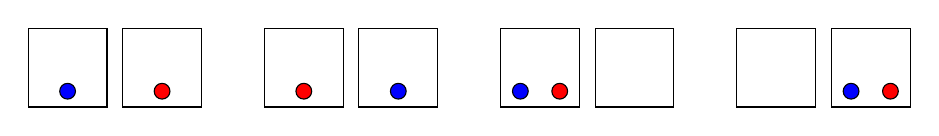
\begin{tikzpicture}
\draw (0,0) rectangle (1,1);
\draw (1.2,0) rectangle (2.2,1);
\draw (3,0) rectangle (4,1);
\draw (4.2,0) rectangle (5.2,1);
\draw (6,0) rectangle (7,1);
\draw (7.2,0) rectangle (8.2,1);
\draw (9,0) rectangle (10,1);
\draw (10.2,0) rectangle (11.2,1);

\draw[fill=blue] (0.5,0.2) circle (0.1);
\draw[fill=red] (1.7,0.2) circle (0.1);
\draw[fill=red] (3.5,0.2) circle (0.1);
\draw[fill=blue] (4.7,0.2) circle (0.1);
\draw[fill=blue] (6.25,0.2) circle (0.1);
\draw[fill=red] (6.75,0.2) circle (0.1);
\draw[fill=blue] (10.45,0.2) circle (0.1);
\draw[fill=red] (10.95,0.2) circle (0.1);
\end{tikzpicture}
\end{center}
در این حالت، امید ریاضی تعداد جعبه‌های خالی برابر است با:
\[\frac{0+0+1+1}{4} = \frac{1}{2}.\]
در حالت کلی، احتمال خالی ماندن یک جعبه خاص برابر است با:
\[\Big(\frac{n-1}{n}\Big)^n,\]
زیرا هیچ توپی نباید درون آن قرار گیرد.
بنابراین با استفاده از خطی بودن امید ریاضی، امید ریاضی تعداد جعبه‌های خالی برابر است با:
\[n \cdot \Big(\frac{n-1}{n}\Big)^n.\]

\subsubsection{توزیع‌ها}

\index{distribution@توزیع}

\key{توزیع} یک متغیر تصادفی $X$، احتمال هر مقداری را که $X$ می‌تواند داشته باشد نشان می‌دهد.
توزیع از مقادیر $P(X=x)$ تشکیل می‌شود.
برای مثال هنگام پرتاب دو تاس، توزیع مجموع آن‌ها برابر است با:
\begin{center}
\small {
\begin{tabular}{r|rrrrrrrrrrrrr}
$x$ & 2 & 3 & 4 & 5 & 6 & 7 & 8 & 9 & 10 & 11 & 12 \\
$P(X=x)$ & $1/36$ & $2/36$ & $3/36$ & $4/36$ & $5/36$ & $6/36$ & $5/36$ & $4/36$ & $3/36$ & $2/36$ & $1/36$ \\
\end{tabular}
}
\end{center}

\index{uniform distribution@توزیع یکنواخت}
در یک \key{توزیع یکنواخت}، متغیر تصادفی $X$ دارای $n$ مقدار ممکن $a,a+1,\ldots,b$ است و احتمال هر مقدار برابر با $1/n$ می‌باشد.
به عنوان مثال، هنگام پرتاب یک تاس، $a=1$ و $b=6$ است و برای هر مقدار $x$ داریم $P(X=x)=1/6$.

امید ریاضی $X$ در یک توزیع یکنواخت برابر است با:
\[E[X] = \frac{a+b}{2}.\]

\index{binomial distribution@توزیع دو‌جمله‌ای}
در یک \key{توزیع دو‌جمله‌ای}، $n$ آزمایش انجام می‌شود و احتمال موفقیت در هر آزمایش برابر با $p$ است.
متغیر تصادفی $X$ تعداد آزمایش‌های موفق را می‌شمارد و احتمال مقدار $x$ برابر است با:
\[P(X=x)=p^x (1-p)^{n-x} {n \choose x},\]
که در آن $p^x$ و $(1-p)^{n-x}$ متناظر با آزمایش‌های موفق و ناموفق هستند، و ${n \choose x}$ بیانگر تعداد روش‌های انتخاب ترتیب آزمایش‌ها است.

برای مثال در ده بار پرتاب یک تاس، احتمال این‌که دقیقاً سه بار عدد شش بیاید برابر است با $(1/6)^3 (5/6)^7 {10 \choose 3}$.

امید ریاضی $X$ در توزیع دو‌جمله‌ای برابر است با:
\[E[X] = pn.\]

\index{geometric distribution@توزیع هندسی}
در یک \key{توزیع هندسی}، احتمال موفقیت در هر آزمایش برابر با $p$ است و تا زمان رخ دادن اولین موفقیت ادامه می‌دهیم.
متغیر تصادفی $X$ تعداد آزمایش‌های لازم را می‌شمارد و احتمال مقدار $x$ برابر است با:
\[P(X=x)=(1-p)^{x-1} p,\]
که در آن $(1-p)^{x-1}$ متناظر با آزمایش‌های ناموفق و $p$ متناظر با اولین آزمایش موفق است.

به عنوان مثال، اگر یک تاس را تا زمانی که عدد شش ظاهر شود پرتاب کنیم، احتمال این‌که تعداد پرتاب‌ها دقیقاً ۴ بار باشد برابر است با $(5/6)^3 1/6$.

امید ریاضی $X$ در یک توزیع هندسی برابر است با:
\[E[X]=\frac{1}{p}.\]

\section{زنجیره‌های مارکوف}

\index{Markov chain@زنجیره مارکوف}

یک \key{زنجیره مارکوف}
% \footnote{A. A. Markov (1856--1922)
% was a Russian mathematician.}
فرآیندی تصادفی شامل مجموعه‌ای از وضعیت‌ها و گذارهای بین آن‌ها است.
به ازای هر وضعیت، احتمال انتقال به وضعیت‌های دیگر معلوم است.
زنجیره مارکوف با گرافی نمایش داده می‌شود
که رأس‌های آن وضعیت‌ها و یال‌های آن گذارها هستند.

به عنوان مثال، مسئله‌ای را در نظر بگیرید
که در طبقه ۱ ساختمانی با $n$ طبقه قرار داریم.
در هر گام، به صورت تصادفی یک طبقه به بالا
یا یک طبقه به پایین می‌رویم، به جز اینکه از طبقه ۱
همیشه یک طبقه بالا رفته و از طبقه $n$ همیشه یک طبقه پایین می‌آییم.
احتمال حضور در طبقه $m$ پس از $k$ گام چقدر است؟

در این مسئله، هر طبقه از ساختمان متناظر با وضعیتی در زنجیره مارکوف است.
مثلاً اگر $n=5$ باشد، گراف به شکل زیر خواهد بود:

\begin{center}
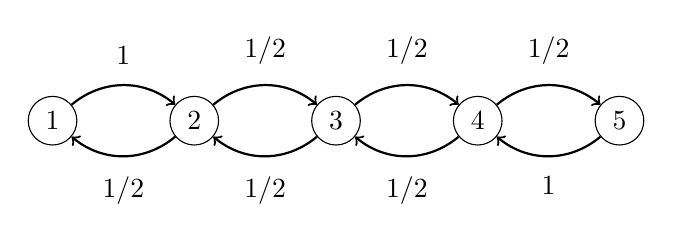
\begin{tikzpicture}[scale=0.9]
\node[draw, circle] (1) at (0,0) {$1$};
\node[draw, circle] (2) at (2,0) {$2$};
\node[draw, circle] (3) at (4,0) {$3$};
\node[draw, circle] (4) at (6,0) {$4$};
\node[draw, circle] (5) at (8,0) {$5$};

\path[draw,thick,->] (1) edge [bend left=40] node[font=\small,label=$1$] {} (2);
\path[draw,thick,->] (2) edge [bend left=40] node[font=\small,label=$1/2$] {} (3);
\path[draw,thick,->] (3) edge [bend left=40] node[font=\small,label=$1/2$] {} (4);
\path[draw,thick,->] (4) edge [bend left=40] node[font=\small,label=$1/2$] {} (5);

\path[draw,thick,->] (5) edge [bend left=40] node[font=\small,label=below:$1$] {} (4);
\path[draw,thick,->] (4) edge [bend left=40] node[font=\small,label=below:$1/2$] {} (3);
\path[draw,thick,->] (3) edge [bend left=40] node[font=\small,label=below:$1/2$] {} (2);
\path[draw,thick,->] (2) edge [bend left=40] node[font=\small,label=below:$1/2$] {} (1);

%\path[draw,thick,->] (1) edge [bend left=40] node[font=\small,label=below:$1$] {} (2);
\end{tikzpicture}
\end{center}

توزیع احتمال زنجیره مارکوف، برداری به صورت
$[p_1,p_2,\ldots,p_n]$ است که در آن $p_k$ بیانگر
احتمال قرار گرفتن در وضعیت $k$ است.
همواره رابطه $p_1+p_2+\cdots+p_n=1$ برقرار است.

در سناریوی بالا، توزیع اولیه برابر با
$[1,0,0,0,0]$ است، چون همیشه از طبقه ۱ شروع می‌کنیم.
توزیع بعدی $[0,1,0,0,0]$ است،
چرا که از طبقه ۱ فقط به طبقه ۲ می‌توان رفت.
پس از آن، می‌توان یا یک طبقه بالا رفت یا یک طبقه پایین،
بنابراین توزیع بعدی برابر با $[1/2,0,1/2,0,0]$ است و به همین ترتیب ادامه می‌یابد.

روشی کارآمد برای شبیه‌سازی حرکت در زنجیره مارکوف، استفاده از برنامه‌نویسی پویا است.
ایده کار نگهداری توزیع احتمال
و در هر گام، بررسی تمام حالت‌های ممکن برای جابه‌جایی است.
با این روش، می‌توان یک مسیر به طول $m$ گام را در زمان $O(n^2 m)$ شبیه‌سازی کرد.

گذارهای زنجیره مارکوف را می‌توان به صورت ماتریسی
نیز نمایش داد که توزیع احتمال را به‌روزرسانی می‌کند.
در سناریوی بالا، این ماتریس به شکل زیر است:

\[ 
 \begin{bmatrix}
  0 & 1/2 & 0 & 0 & 0 \\
  1 & 0 & 1/2 & 0 & 0 \\
  0 & 1/2 & 0 & 1/2 & 0 \\
  0 & 0 & 1/2 & 0 & 1 \\
  0 & 0 & 0 & 1/2 & 0 \\
 \end{bmatrix}.
\]

وقتی یک توزیع احتمال را در این ماتریس ضرب کنیم،
توزیع جدید پس از یک گام حرکت به دست می‌آید.
برای نمونه، می‌توان از توزیع
$[1,0,0,0,0]$ به توزیع
$[0,1,0,0,0]$ به صورت زیر رفت:

\[ 
 \begin{bmatrix}
  0 & 1/2 & 0 & 0 & 0 \\
  1 & 0 & 1/2 & 0 & 0 \\
  0 & 1/2 & 0 & 1/2 & 0 \\
  0 & 0 & 1/2 & 0 & 1 \\
  0 & 0 & 0 & 1/2 & 0 \\
 \end{bmatrix}
 \begin{bmatrix}
  1 \\
  0 \\
  0 \\
  0 \\
  0 \\
 \end{bmatrix}
=
 \begin{bmatrix}
  0 \\
  1 \\
  0 \\
  0 \\
  0 \\
 \end{bmatrix}.
\]

با محاسبه توان‌های ماتریس به شکل بهینه،
می‌توان توزیع پس از $m$ گام را
در زمان $O(n^3 \log m)$ محاسبه کرد.

\section{الگوریتم‌های تصادفی}

\index{randomized algorithm}

گاهی می‌توان از تصادف برای حل مسئله استفاده کرد،
حتی اگر مسئله ربطی به احتمال نداشته باشد.
یک \key{الگوریتم تصادفی} الگوریتمی است که
بر پایه تصادف کار می‌کند.

\index{Monte Carlo algorithm}

یک \key{الگوریتم مونت‌کارلو} الگوریتمی تصادفی است
که ممکن است گاهی پاسخ نادرست بدهد.
برای کاربردی بودن چنین الگوریتمی،
احتمال پاسخ نادرست باید کم باشد.

\index{Las Vegas algorithm}

یک \key{الگوریتم لاس‌وگاس} الگوریتمی تصادفی است
که همیشه پاسخ درست می‌دهد،
ولی زمان اجرای آن به صورت تصادفی تغییر می‌کند.
هدف طراحی الگوریتمی است که
با احتمال بالا کارآمد باشد.

در ادامه به سه مسئله نمونه می‌پردازیم که
با تصادف حل می‌شوند.

\subsubsection{آماره‌های ترتیبی}

\index{order statistic}

$k$-امین \key{آماره ترتیبی} در یک آرایه،
عنصر واقع در موقعیت $k$ پس از مرتب‌سازی
صعودی آرایه است.
محاسبه هر آماره ترتیبی با مرتب‌سازی اولیه آرایه
در زمان $O(n \log n)$ آسان است،
ولی آیا واقعاً مرتب‌سازی کل آرایه
فقط برای یافتن یک عنصر لازم است؟

مشخص می‌شود می‌توان آماره‌های ترتیبی را
با الگوریتم تصادفی بدون مرتب‌سازی آرایه یافت.
این الگوریتم، معروف به \key{انتخاب سریع}\footnote{در سال ۱۹۶۱،
سی. ای. آر. هاور دو الگوریتم معرفی کرد که
در حالت میانگین کارآمد هستند: \index{quicksort} \index{quickselect}
\key{مرتب‌سازی سریع} \cite{hoa61a} برای مرتب‌سازی آرایه‌ها و
\key{انتخاب سریع} \cite{hoa61b} برای یافتن آماره‌های ترتیبی.}، یک الگوریتم لاس‌وگاس است:
زمان اجرای آن معمولاً $O(n)$ است
ولی در بدترین حالت $O(n^2)$ می‌شود.

الگوریتم یک عنصر تصادفی $x$
از آرایه انتخاب می‌کند، و عناصر کوچک‌تر از $x$ را
به بخش چپ آرایه منتقل می‌کند،
و سایر عناصر را به بخش راست آرایه می‌برد.
این کار در حضور $n$ عنصر، زمان $O(n)$ می‌برد.
فرض کنید بخش چپ شامل $a$ عنصر
و بخش راست شامل $b$ عنصر باشد.
اگر $a=k$ باشد، عنصر $x$ همان $k$-امین آماره ترتیبی است.
در غیر این صورت، اگر $a>k$ باشد، به شکل بازگشتی $k$-امین آماره
ترتیبی را برای بخش چپ پیدا می‌کنیم،
و اگر $a<k$ باشد، به شکل بازگشتی $r$-امین آماره
ترتیبی را برای بخش راست می‌یابیم که در آن $r=k-a$ است.
جستجو به همین ترتیب ادامه می‌یابد تا عنصر
پیدا شود.

وقتی هر عنصر $x$ تصادفی انتخاب شود،
اندازه آرایه در هر مرحله تقریباً نصف می‌شود،
بنابراین پیچیدگی زمانی برای
یافتن $k$-امین آماره ترتیبی تقریباً برابر است با
\[n+n/2+n/4+n/8+\cdots < 2n = O(n).\]

بدترین حالت الگوریتم همچنان به زمان $O(n^2)$ نیاز دارد،
زیرا ممکن است $x$ همواره به گونه‌ای انتخاب شود
که یکی از کوچک‌ترین یا بزرگ‌ترین عناصر آرایه باشد
و به $O(n)$ مرحله نیاز شود.
با این حال، احتمال وقوع این حالت آن‌قدر کم است
که در عمل هرگز رخ نمی‌دهد.

\subsubsection{بررسی درستی ضرب ماتریس‌ها}

\index{matrix multiplication}

مسئله بعدی ما \emph{بررسی} این است
که آیا رابطه $AB=C$ برقرار است یا خیر، در حالی که $A$، $B$ و $C$
ماتریس‌هایی با اندازه $n \times n$ هستند.
البته می‌توان مسئله را با محاسبه دوباره
حاصل‌ضرب $AB$ حل کرد
(در زمان $O(n^3)$ با استفاده از الگوریتم پایه)،
اما انتظار می‌رود که بررسی درستی پاسخ
آسان‌تر از محاسبه آن از ابتدا باشد.

مشخص می‌شود که می‌توان مسئله را با
یک الگوریتم مونت‌کارلو\footnote{آر. ام. فرایوالدز این الگوریتم را در سال ۱۹۷۷ منتشر کرد \cite{fre77}، و گاهی
\index{Freivalds' algoritm} \key{الگوریتم فرایوالدز} نامیده می‌شود.} حل کرد که
پیچیدگی زمانی آن تنها $O(n^2)$ است.
ایده ساده است: بردار تصادفی $X$
شامل $n$ عنصر را انتخاب می‌کنیم و ماتریس‌های
$ABX$ و $CX$ را محاسبه می‌نماییم. اگر $ABX=CX$ باشد، اعلام می‌کنیم $AB=C$،
و در غیر این صورت گزارش می‌دهیم $AB \neq C$.

پیچیدگی زمانی الگوریتم
$O(n^2)$ است، زیرا می‌توان ماتریس‌های
$ABX$ و $CX$ را در زمان $O(n^2)$ محاسبه کرد.
می‌توان ماتریس $ABX$ را با استفاده از نمایش $A(BX)$ بهینه محاسبه کرد،
بنابراین تنها به دو ضرب ماتریس
با اندازه‌های $n \times n$ و $n \times 1$ نیاز است.

نقطه ضعف الگوریتم این است
که احتمال کمی وجود دارد که هنگام اعلام $AB=C$ دچار خطا شود.
برای مثال،
\[
 \begin{bmatrix}
  6 & 8 \\
  1 & 3 \\
 \end{bmatrix}
\neq
 \begin{bmatrix}
  8 & 7 \\
  3 & 2 \\
 \end{bmatrix},
\]
اما
\[
 \begin{bmatrix}
  6 & 8 \\
  1 & 3 \\
 \end{bmatrix}
 \begin{bmatrix}
  3 \\
  6 \\
 \end{bmatrix}
=
 \begin{bmatrix}
  8 & 7 \\
  3 & 2 \\
 \end{bmatrix}
 \begin{bmatrix}
  3 \\
  6 \\
 \end{bmatrix}.
\]
با این حال در عمل، احتمال خطای الگوریتم اندک است،
و می‌توان این احتمال را با بررسی نتیجه با چندین
بردار تصادفی $X$ پیش از اعلام $AB=C$، کاهش داد.

\subsubsection{رنگ‌آمیزی گراف}

\index{coloring}

با فرض داشتن گرافی شامل $n$ رأس و $m$ یال،
وظیفه ما یافتن روشی برای رنگ‌آمیزی رأس‌های
گراف با دو رنگ است به طوری که
حداقل برای $m/2$ یال، دو سر یال دارای
رنگ‌های متفاوتی باشند.
برای مثال، در گراف
\begin{center}
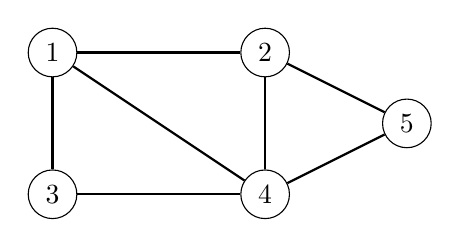
\begin{tikzpicture}[scale=0.9]
\node[draw, circle] (1) at (1,3) {$1$};
\node[draw, circle] (2) at (4,3) {$2$};
\node[draw, circle] (3) at (1,1) {$3$};
\node[draw, circle] (4) at (4,1) {$4$};
\node[draw, circle] (5) at (6,2) {$5$};

\path[draw,thick,-] (1) -- (2);
\path[draw,thick,-] (1) -- (3);
\path[draw,thick,-] (1) -- (4);
\path[draw,thick,-] (3) -- (4);
\path[draw,thick,-] (2) -- (4);
\path[draw,thick,-] (2) -- (5);
\path[draw,thick,-] (4) -- (5);
\end{tikzpicture}
\end{center}
یک رنگ‌آمیزی معتبر به صورت زیر است:
\begin{center}
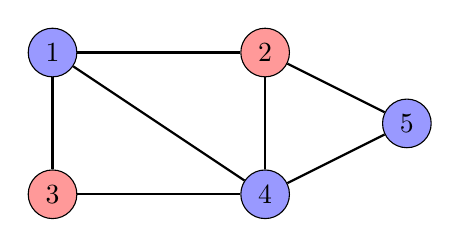
\begin{tikzpicture}[scale=0.9]
\node[draw, circle, fill=blue!40] (1) at (1,3) {$1$};
\node[draw, circle, fill=red!40] (2) at (4,3) {$2$};
\node[draw, circle, fill=red!40] (3) at (1,1) {$3$};
\node[draw, circle, fill=blue!40] (4) at (4,1) {$4$};
\node[draw, circle, fill=blue!40] (5) at (6,2) {$5$};

\path[draw,thick,-] (1) -- (2);
\path[draw,thick,-] (1) -- (3);
\path[draw,thick,-] (1) -- (4);
\path[draw,thick,-] (3) -- (4);
\path[draw,thick,-] (2) -- (4);
\path[draw,thick,-] (2) -- (5);
\path[draw,thick,-] (4) -- (5);
\end{tikzpicture}
\end{center}
گراف بالا دارای ۷ یال است و برای ۵ تای آن‌ها،
دو سر یال رنگ‌های متفاوتی دارند،
بنابراین رنگ‌آمیزی معتبر است.

مسئله را می‌توان با الگوریتم لاس‌وگاس حل کرد
که رنگ‌آمیزی‌های تصادفی تولید می‌کند تا زمانی که رنگ‌آمیزی معتبر
یافت شود.
در رنگ‌آمیزی تصادفی، رنگ هر رأس به‌طور
مستقل انتخاب می‌شود به‌طوری که احتمال
هر دو رنگ برابر $1/2$ است.

در رنگ‌آمیزی تصادفی، احتمال اینکه دو سر
یک یال رنگ‌های متفاوت داشته باشند $1/2$ است.
بنابراین، امید ریاضی تعداد یال‌هایی که دو سر آن‌ها
رنگ‌های متفاوت دارند $m/2$ است.
از آنجا که انتظار می‌رود رنگ‌آمیزی تصادفی معتبر باشد،
در عمل خیلی سریع رنگ‌آمیزی معتبر پیدا می‌کنیم.